\documentclass[10pt,twocolumn,letter]{article}
\usepackage{styles/usenix-style}
\usepackage{styles/ka-style}
\usepackage{xspace,ifthen,graphicx,listings}
\usepackage{styles/ka-style}

\usepackage[utf8]{inputenc}
\usepackage[inline]{enumitem}
\usepackage{parskip} % disable indentation for new paragraphs, increased margin-bottom instead
\usepackage[english]{babel}
\usepackage{csquotes}
\usepackage[style=alphabetic]{biblatex}
\addbibresource{literature.bib}

\usepackage[
   pdfauthor={Christian Schwarz},
   pdftitle={Seminar Report - Light-Weight Contexts},
   pdfsubject={An OS Abstraction for Safety and Performance}, 
   pdfkeywords={}
]{hyperref}

\setlength{\marginparwidth}{2cm} % to make todonotes fit in twocolumn
\usepackage{todonotes}

\usepackage{blindtext}

\usepackage{listings}
\lstdefinestyle{lwcapi}{language=[ANSI]C,basicstyle=\ttfamily,basewidth=0.5em,fontadjust=true}
\lstset{style=lwcapi}

\usepackage{diagbox}
\usepackage{multirow}

\begin{document}
\title{%
  % document class article doesn't support subtitles, let's hack them
  {\normalfont \normalsize Seminar Report on}\\%
  Light-weight Contexts\\%
  {\normalfont \normalsize An OS Abstraction for Safety and Performance}\\%
  {\normalfont \small %
    James Litton\textsuperscript{1,2}
    Anjo Vahldiek-Oberwagner\textsuperscript{2}
    Eslam Elnikety\textsuperscript{2}
    Deepak Garg\textsuperscript{2}
    Bobby Bhattacharjee\textsuperscript{1}
    Peter Druschel\textsuperscript{2}
  }\\
  {\normalfont \small
    \textsuperscript{1}University of Maryland, College Park 
    \textsuperscript{2}Max Planck Institute for Software Systems
  }%
}
\author{Report by Christian Schwarz}
\date{2019}

\maketitle

\begin{abstract}
  \blindtext\todo{fix blindtext}
\end{abstract}

\section{Introduction}\label{intro}

% TODO NICE SUMMARY OF WHAT LWCs PROVIDE, CAN WE USE THIS ANYWHERE?
%Light-weight contexts can be used to create multiple protection domains within a single process,
%each with a private \textit{address space}, \textit{file descriptor table} and the system \textit{credential} and private per-thread logical control-flow %state (section~\ref{design:createdestroy}).
%Switching between the domains and single-value argument passing is controlled by the kernel (section~\ref{design:switching}).
%Dynamic sharing of resources between lwCs is also kernel-controlled using access capabilities (section~\ref{design:overlays}).
%Access to global namespaces \& system resources (IP sockets, filesystem, IPC) is limited by the lwC's \textit{credential} and can be further controlled %through syscall interposition (section~\ref{design:syscallinterpos}).
%
%Kernel-controlled switching between lwCs results in \textbf{well-defined entry points} under the assumption of an lwC created using \lstinline{COPY} resource %specifier\todo{this is quite coarse, AS and FDT sufficient?}:
%the first \lstinline{lwcSwitch} diverts physical control flow to the \lstinline{lwcCreate} call site in the new lwC, and all subsequent \lstinline{lwcSwitch}%es resume execution at an lwcSwitch all site.
%Under the assumption of no dynamic sharing, the address space of the target lwC is inaccessible to any caller.
%Thus, integrity and confidentiality guarantees for code and data within an lwC are those of the application code creating the lwC and those of the code %executing in the target lwC after \lstinline{lwcSwitch}.
%The result is a narrow, auditable interface.
%

Application Compartmentalization as in seminar presentation. Ignore Session Isolation \& Snapshots?

Line of throught:

Modern app architecture commonly emphasizes modularization \& information hiding (Parnas) to achieve testability, maintainability, exchangability, reusability.
The extreme of reusability are large libraries used by multiple independent applications.

However, chasm between development time and runtime:
PLs enforce encapsulation at compile time, but the resulting program runs in a single protection domain, i.e. a process, at runtime:
shared address space with shared heap, shared file descriptor table, shared system-level privilege (user id, group id, capabilities(SYS\_CAP\_), system call) between all modules of the program.
Consequently, an exploitable vulnerability in a single module not only compromises that module but the entire application.

The generic solution: decomponsition of the application into smaller units that execute in separate protection domains.
Generic questions / problems / tradeoffs:
\begin{itemize}
  \item threat model
  \item definition of what makes a protection domain
  \item how to integrate the decomposition into different protection domains into the PL / runtime?
  \item applicability to existing PLs \& code bases
  \item how to maintain application performance
\end{itemize}

\subsection{Structure of this Report}
\blindtext\todo{fix blindtext}


\section{Design}\label{design}
We find it most helpful to develop the general idea of \textit{light-weight Contexts} (lwCs) by starting from the canonical abstraction of processes \& threads, as visualized in figure~\ref{design:fig:canonicalprocthreads}.
\begin{figure}
  \label{design:fig:canonicalprocthreads}
  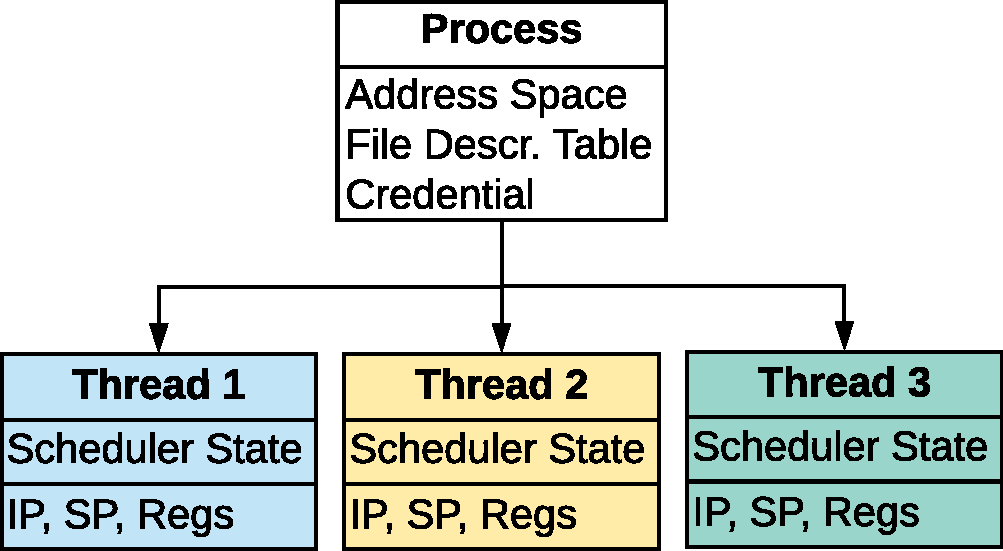
\includegraphics[width=\linewidth]{fig/canonical-proc-thread-relationship}
  \caption{
    Canonical state associated with processes and threads and the relationship between them.
    The process implicitly defines the execution environment for threads.
    Threads are scheduling entities that represent a single control flow bound to the process-defined environment.
  }
\end{figure}
Conventionally, processes define an execution environment which is shared by one or more threads.
The execution environment consists of an address space, a file descriptor table and a representation of the process's system-wide privileges (\textit{credential}).
A thread has \textbf{two closely related, but separate roles}:
\textbf{first}, it represents a \textbf{single unit of logical control flow} within the process-defined environment.
Control flow has associated state, e.g., instruction pointer, stack pointer, general purpose register contents, FPU state, etc.
That state resides in a CPU's registers while the thread is executing on a CPU, or in the thread control block (TCB) kernel data structure.
The \textbf{second} role of a thread is that of a \textbf{scheduling entity}:
The scheduler time-multiplexes threads onto CPU cores and implements the concept of blocking \& waiting between threads.
The scheduler state required for this task is stored in the thread control block (TCB).

The authors introduce light-weight contexts as a new OS abstraction and restructure the roles of canonical processes \& threads, as visualized in figure~\ref{design:fig:lwcprocthreadrelationship}:

\begin{figure}[h]
  \label{design:fig:lwcprocthreadrelationship}
  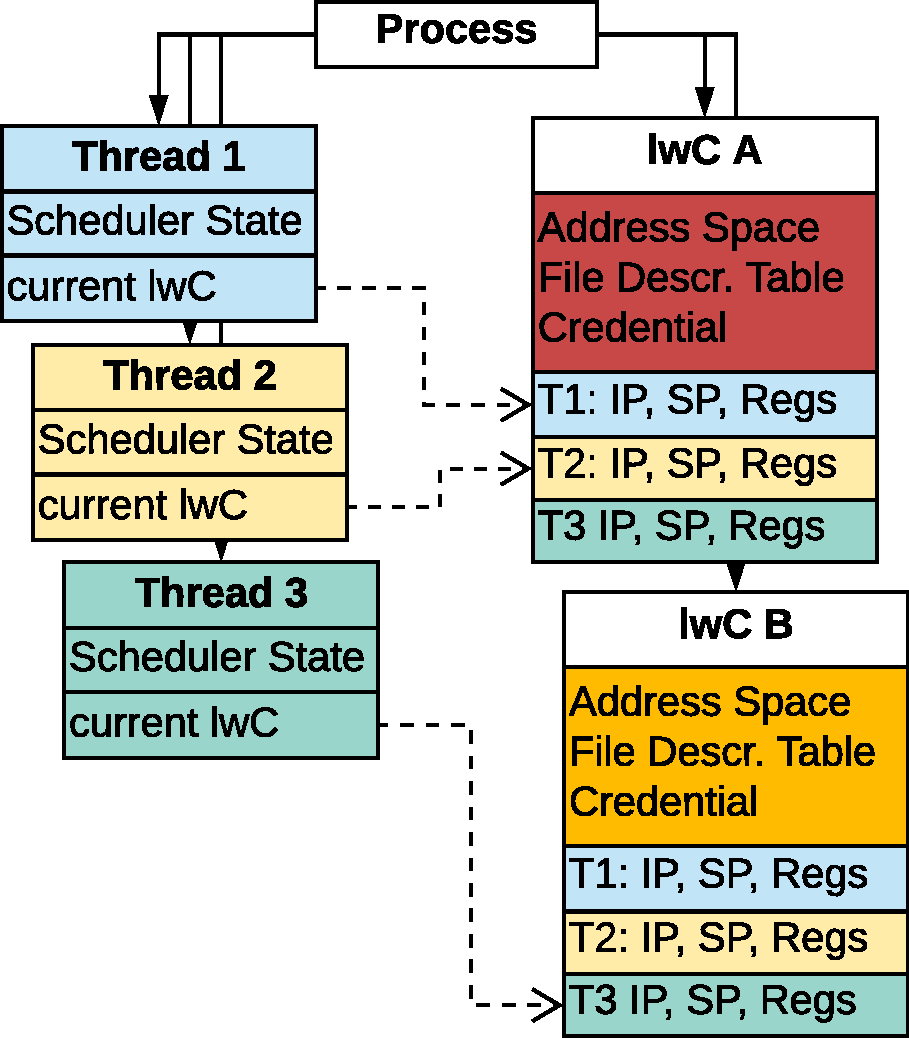
\includegraphics[width=\linewidth]{fig/lwc-proc-thread-relationship}
  \caption{
    State associated with lwCs, processes and threads and relationships between them.
    Processes act as containers for threads and lwCs.
    Threads are reduced to their role as scheduling entities.
    Each lwC represents an execution environment and holds control flow state for each thread.
  }
\end{figure}

\begin{itemize}
\item An lwC represents a single protection domain (address space, file descriptor table and system credential) and all logical control flows within that protection domain.
\item Threads always execute within one lwC at any given time and always execute the same logical control flow while within that lwC.
\item Multiple threads can execute simultaneously within an lwCs, sharing a protection domain but executing different logical flows.
\item lwCs are represented as file descriptors, and thus explicitly tangible from user space.
\item Threads can switch protection domains and logical control flow by switching between lwCs.
\end{itemize}

In the following subsections, we provide an outline of the system API for managing and using lwCs in an application.
Subsequently, we summarize the security guarantees provided by lwCs and provide usage examples for this new OS abstraction. 

\subsection{lwC Switching}\label{design:switching}
We start our survey of the lwC API surface with the most central functionality: switching between lwCs.
We accept the existence of multiple lwCs for now and come back to lwC creation in the next subsection.

Threads can switch between lwCs by invoking the \lstinline{lwcSwitch} system call:

\begin{lstlisting}[float=h]
  caller, carg := lwcSwitch(target, arg) 
\end{lstlisting}

The first argument \lstinline{target} specifies the file descriptor of the lwC into which the calling thread wants to switch.
When invoking the system call, the kernel
\begin{enumerate}[label=(\alph*)]
\item saves the current control flow state into the current thread's lwC,
\item atomically switches to the new protection domain by installing the target lwC address space, file descriptor table and credential for the current thread,
\item and restores the control flow state saved for the current in thread in the target lwC.
\end{enumerate}
Pseudo code for this procedure is provided in listing~\ref{design:fig:switchpseudocode}.

\begin{lstlisting}[mathescape,label=design:fig:switchpseudocode,caption=Pseudo code for lwcSwitch.,frame=trbl]
  syscall
  
  SP, IP, $\dots$ $\rightarrow$ curLWC->tcb[tid]
  
  curThd->vmspace = targetLWC->vmspace
  curThd->fdt = targetLWC->fdt
  curThd->cred = targetLWC->cred
  curLWC = targetLWC
  
  SP, IP, $\dots$ $\leftarrow$ targetLWC->tcb[tid]
  (arg kept in register)
  
  sysret  
\end{lstlisting}
  
It is crucial to understand that \textbf{execution after a switch always resumes at an lwC call site}, except for the very first switch into a newly created lwC (see section~\ref{design:createdestroy}).
Note that this behavior is analogous to a voluntary context switch, e.g., with \lstinline{pthread_yield}.
However, in contrast to the canonical model of processes \& threads, \textbf{\lstinline{lwcSwitch} does not switch to another scheduling entity}:
from the thread scheduler's perspective, it is still the same thread that is executing on the CPU.
In fact, \textbf{the thread scheduler is not affected at all by lwC switching}:
it still handles context switches post-interrupt, post-exception or when a thread blocks, by simply saving that thread's control flow state to the slot in the current lwC before switching to another thread (i.e.~scheduling entity).

The second argument to \lstinline{lwcSwitch} is an opaque value called \lstinline{arg} that is passed through to the code that starts executing in the target lwC after the switch is completed.
\lstinline{arg} is made available in the target lwC as the return value \lstinline{carg} (we remember that execution always resumes at an lwC call site).
The second return value \lstinline{caller} is the file descriptor of the lwC from where the switch was initiated.
Having this information available in the switch target enables subroutine-style usage of \lstinline{lwcSwitch} because it enables switching back to any number of callers that are unknown at compile time.

% do not mention coroutines here, will do that in the application

\subsection{lwC Creation \& Destruction}\label{design:createdestroy}
A process in an lwC system starts with a single thread that runs within a root lwC created by the OS.
This design enables backwards binary-compatiblity with the exception that the root lwC file descriptor is a well-known number analogous to those for stdio.

New lwCs can then be created by threads using the \lstinline{lwcCreate} system call:

\begin{figure}[h]
  \centering
\begin{lstlisting}[mathescape]
  new, caller, carg := lwcCreate(rspecs)
\end{lstlisting}
\begin{tabular}{|r||c|c|c|}
  \hline
                &   new        & caller       & carg \\
  \hline\hline
  creator       & new lwC fd   & $\bot$      & $\bot$\\
  \hline
  new lwC       &    creator lwC fd   & \multicolumn{2}{c|}{like lwcSwitch}\\
  \hline
\end{tabular}
\caption{
  \texttt{lwcCreate} return values are different in creator and new lwC to ensure well-defined behavior when the creator switches to the new lwC for the first time.
}
\end{figure}

By default, a new lwC is a snapshot of the calling thread's current lwC, as depicted in figure~\ref{design:fig:lwccreationsequencediagram}:
The kernel first creates copies of the resources \textit{address space}, \textit{file descriptor table} and \textit{credentials} and stores them in the new lwC.
It then temporarily preempts all threads that execute in the current lwC and stores their control flow state in the new lwC.
The execution state of other threads that can switch to the creating lwCs is simply copied to the new lwC.
Finally, the file descriptor referring to the new lwC is returned to user space in the return value \lstinline{new}.

\begin{figure}
  \centering
  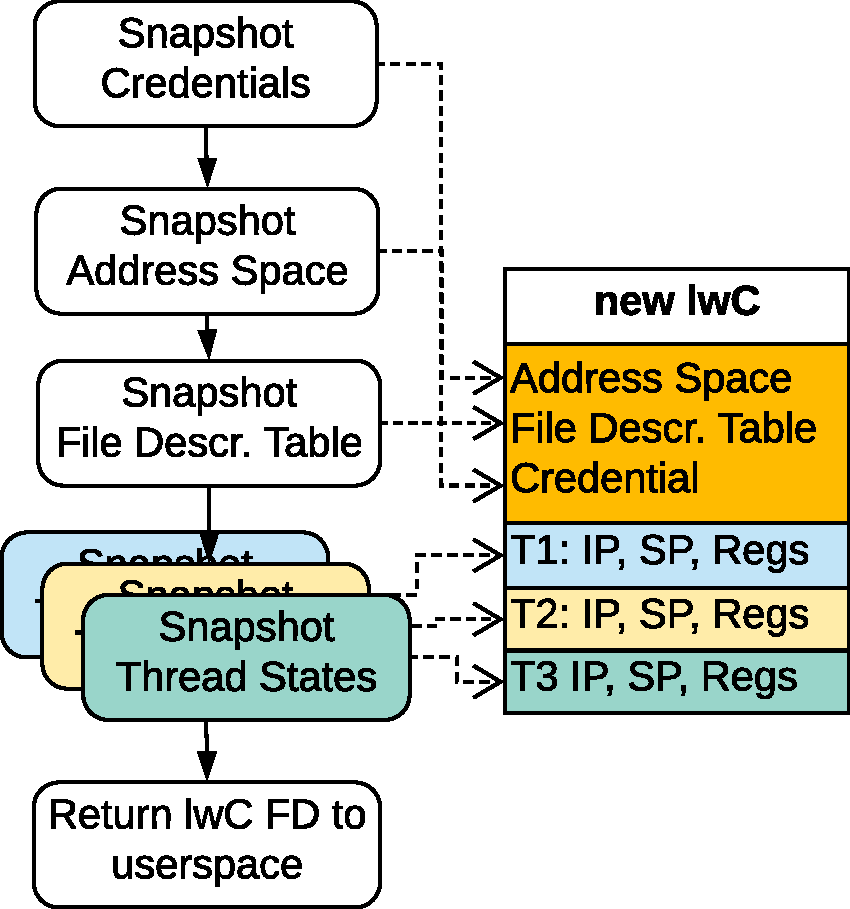
\includegraphics[height=4cm]{fig/lwc-creation-sequence-diagram}
  \caption{
    Steps involved in lwC creation.
    By default, a new lwC is a copy (snapshot) of the current lwC's resources.
    All threads that exist at the time of lwC creation can enter the new lwC.
  }
\label{design:fig:lwccreationsequencediagram}
\end{figure}

Note that in contrast to the original paper, we avoid the term \textit{fork} when describing the lwC creation procedure:
forking has the same resource snapshotting semantics as \textit{lwcCreate}, but also implies the creation of a new process and scheduling entity.
In contrast, \textit{lwcCreate} only creates a copy of the protection domain and a handle for existing threads to switch to it later --- no independent scheduling entity is created.

However, one problem of forking translates to lwC creation:
\textbf{what happens when we first switch into a newly created lwC? How does snapshotting interact with multi-threading?}
After all, we preempt and snapshot all threads' control flow states on lwC creation, and the \lstinline{lwcSwitch} implementation restores that state on first switch, expecting that it was an \lstinline{lwcSwitch} call site.
We need to consider two cases:
the \lstinline{lwcCreate}ing thread will appear return "a second time" from that syscall and populate \lstinline{lwcCreate}'s \lstinline{caller} and \lstinline{carg} return values with those of \lstinline{lwcSwitch}.
Additionally, the \lstinline{new} contains the lwC descriptor of the creator lwC.
The behavior in the creating thread is thus well-defined.
Other threads could be at random points in their logical control flow when being snapshotted, resulting in undefined behavior after the switch.\todo{obvious?}
Multithreaded forking is a well-known problem, \todo{citation} and the authors recommend applications to use barrier-synchronization with the creator.\todo{cite}
However, it is unclear to us how the \lstinline{caller} and \lstinline{carg} return values are accessible without inline-assembly or language support for non-creator threads.\todo{check}

Finally, it should be noted that a new lwC only stores control flow states for the threads that existed at the time of its creation:
threads created after the lwC cannot switch into the lwC.

\subsubsection{lwC Resource Specifiers}\label{design:rspecs}
The previous section presented the default behavior of \lstinline{lwcCreate} for an empty \lstinline{rspecs} argument, which amounts to the new lwC being a snapshot copy of the current lwC's \textbf{resources} \textit{address space}, \textit{file descriptor table} and \textit{credential}.
By using \textit{resource specifiers}, the application can control resource sharing at a more fine-grained level:
resources of the current lwC can be either \textit{copied to}, \textit{unmapped from} or \textit{shared} with the new lwC.
For address space and file descriptors, different sharing behavior can be specified on a per-page or per-descriptor basis.
Figure~\ref{design:fig:rspectable} summarizes the different combinations of resources and sharing behavior.

\begin{figure}[h]
  \centering
\begin{lstlisting}
rspecs := [{Resource , [Start, End), How}]
\end{lstlisting}

\begin{tabular}{|r||m{1.5cm}|m{1.5cm}|m{1.5cm}|}
  \hline
  \diagbox[width=5em]{How}{What}    &     Address Space         &         File Descriptor Table         &           Credential           \\
  \hline
  COPY                              &   copy on write sharing           &      \texttt{dup} open FDs once    &  copy credential kobject  \\
  \hline              
  UNMAP                             &   do not map              &       do not \texttt{dup} FDs         &    $\bot$       \\
  \hline              
  SHARE                             &   shared memory            &   share kobject   &             share kobject   \\
  \hline
\end{tabular}
\caption{
  Resource specifiers change the default snapshot semantics of \texttt{lwcCreate}:
  each resource can be copied, shared or unmapped from the new lwC.
  Address space and file descriptor sharing can be configured per page / per descriptor.
  \textit{copy} sharing is roughly equivalent to what happens on \texttt{fork}, \textit{share} to what happens on thread creation.
  }
\label{design:fig:rspectable}
\end{figure}
\todo{language, prettier table}

\subsection{Dynamic Resource Sharing with lwC Overlays \& Access Capabilities}\label{design:overlays}
Apart from sharing at lwC creation time, it is also possible to dynamically copy or share memory and file descriptors between lwCs or to temporarily escalate system privileges to the credential of another lwC through the \lstinline{lwcOverlay(src, rspecs)} system call.
The \lstinline{src} argument is the file descriptor of the lwC from which the subset of resources specified in \lstinline{rspecs} should be mapped (\textit{overlaid}) into the current lwC.
The target address (for memory overlays) or file descriptor number is guaranteed to be the same as in \lstinline{src}.
To unmap an existing overlay, \lstinline{src} must be set to the current lwC and \lstinline{rspecs} must be filled with \lstinline{UNMAP} resource specifiers. 
Overlays do not support stacking: after unmapping an overlay that overlaid an existing memory mapping, that original memory mapping is not automatically remapped.\todo{proof by code}  %vmspace_lwc_merge

Overlaying resources from an lwC descriptor \lstinline{src} further requires that this descriptor is equipped with \textbf{access capabilities} for each requested resource.
The rules of this capability system are as follows:
\begin{itemize}
  \item After lwC creation, the creator receives the \lstinline{new} lwC descriptor with a universal access capability to the child lwC.
  \item After lwC creation, the child receives the lwC descriptor of its creator in \lstinline{new}, equipped with access capabilities to ranges flagged with \lstinline{LWC_MAY_ACCESS} on lwcCreate.
  \item Access capabilities cannot be extended.
  \item Access capabilities can be reduced with the \lstinline{lwcRestrict(target, rspecs)} system call by any lwC that holds the lwC descriptor \lstinline{target}:
        after a successful \lstinline{lwcRestrict}, the resource ranges specified in \lstinline{rspecs} can no longer be overlaid using \lstinline{lwcOverlay(target, ...)}.
  \item Access capabilities are invariant across overlays: to the file descriptor entry in the kernel, and is therefore invariant across overlays.
\end{itemize}

In order to grasp the access capability system, we find it helpful to peek at the authors' implementation.
The access capabilities associated with an lwC descriptor are represented as an \lstinline{rspecs} in lwC file descriptor table entry (\lstinline{struct filedescent}).
The overlay permission check enforces that the requested overlay rspec is a subset of the rspec in that file descriptor table entry.

Note that revocation of existing overlays is not possible, i.e., \lstinline{lwcRestrict} only affects future overlays.\todo{proof, not mentioned in paper / impl. see microkernel discussions}

\subsection{Syscall Interposition in Capability Mode}\label{design:syscallinterpos}
% kernel: lwctrapto in sys/kern/subr_syscall.c basically just calls lwcswitch 
When compartmentalizing an application into different lwCs, it can be desirable to limit the system calls an lwC may perform, e.g., to limit filesystem access to a subdirectory or prohibit network communication.
The lwC design builds onto existing syscall filtering and mechanisms, e.g. Capsicum capability mode on FreeBSD or seccomp on Linux\todo{cite}:
when an lwC is created with the \lstinline{LWC_TRAP_SYSCALL} flag, system calls made by the new lwC or any of its children that would normally trap due to the syscall filtering mechanism are redirected to the creator as an \lstinline{lwcSwitch} with \lstinline{caller} set to the trapping lwC.
After the trap-handling lwC has evaluated its policy, the \lstinline{lwcSyscall} system call provides the mechanism for the trap-handling lwC to execute any system call (the original one, another one) \textbf{in the context of the trapping lwC}:

\begin{lstlisting}[float=h]
  lwcSyscall(trappingLwc, mask,
             syscall, syscall-args)
\end{lstlisting}

An alternative design could require the trap-handling lwC to invoke the allowed syscalls itself and return the result as the opaque argument in an \lstinline{lwcSwitch} to the trapping lwC.
However, if the syscall arguments contain pointers to user memory or file descriptors, the trap-handling lwC would need to overlay those from the trapping lwC.
\lstinline{lwcSyscall} avoids the associated overhead:
the \lstinline{mask} argument allows the trap-handling lwC to choose per resource type\footnote{granularity: all memory, all file descriptors, the credential} whether its own mapping or that of the trapping lwC should be used while the syscall is executed.


\subsection{Signal Delivery}
UNIX signal delivery with lwCs faces the same design questions as with threads, i.e., to which lwCs a given signal should be delivered.
The authors' solution is to classify signals as either \textit{attributable} or \textit{non-attributable}:
attributable signals such as for segmentation faults are always delivered to the thread in the lwC that caused the signal to occur.
Non-attributable signals are delivered to \textit{all} lwCs created with a corresponding flag.
Consequently, each thread must have a separate signal mask per lwC.\todo{verify in src}

\subsection{Forking \& Exit}
A forked process inherits the parent's lwCs.
However, only the forking thread exists in the child process, presumably due to POSIX compliance\cite{forkmultithread}. %read do_fork, which calls copy_snaps
Shared memory, either through resource-specifiers on \lstinline{lwcCreate} or \lstinline{lwcOverlay} or through \lstinline{mmap(..., MAP_SHARED)} stays shared accross forks.
The authors do not specify the behavior for file descriptor tables and credential; we assume unmodified fork semantics per lwC.

\subsection{Summary}

\todo{TODO}
% TODO TODO TODO TODO TODO TODO TODO TODO TODO TODO TODO TODO TODO TODO TODO TODO TODO TODO TODO TODO TODO TODO TODO TODO 
\begin{figure}[h] % TODO make this a broad figure?
\centering
\begin{tabular}{|r|m{1.5cm}|}
  \hline
  lwcCreate & \\
  \hline
  lwcClose & \\
  \hline
  lwcGetLwc & \\
  \hline
  lwcSwitch &  \\
  \hline
  lwcOverlay & \\
  \hline
  lwcRestrict & \\
  \hline
  lwcSyscall & \\
  \hline
\end{tabular}
  \caption{lwc API summary table}
\end{figure}


\section{Security Analysis}\label{design:threat}

In this section, we define a threat model for lwCs and assess how the design meets the canonical information security properties of \textit{confidentiality}, \textit{integrity} and \textit{availability}\cite{ciagoals}.

\textbf{Threat Model}\hspace{1em}
The run-time trusted computing base of a process that uses light-weight contexts is the
hardware,
firmware,
monolithic OS kernel,
any user space processes able to influence the execution \& environment of the lwC-process,
and any user space code that runs before \lstinline{main} starts executing.
Once \lstinline{main} starts executing, we assume an attacker who is able to hijack control flow and execute arbitrary code in user-mode in the currently established execution context, i.e., the current lwC.
Specifically, an attacker may access any mapped memory through unprivilieged instructions and invoke any system call, including lwC management calls, and attempt privilege escalation directly or indirectly by invoking said system calls.

\textbf{Resource Mappings}\hspace{1em}
An lwC consists of resource mappings for the three resource kinds address space, file descriptor table and credential.
The kernel implementation of \texttt{lwcSwitch} must guarantee that all kernel subsystems as well as the memory management unit will always perform their respective access permission checks against the resource mappings of the lwC that was last switched to, i.e., the current thread's current lwC.
Under that assumption, the lwC security guarantees rely solely on the soundness of the rules by which resource mappings can be manipulated from user space through \lstinline{lwcCreate}, \lstinline{lwcRestrict} and \lstinline{lwcOverlay}, as well as their correct implementation.
Note that neither the original paper's authors nor us provide a proof of soundness of the resource mapping manipulation.

The \lstinline{lwcSyscall} API must be considered separately:
its \lstinline{mask} argument allows the trap-handling lwC to specify a \textit{subset} of resource mappings to be established for the duration of the syscall.
This differs from \lstinline{lwcSwitch}, which only allows switching \textit{all three resource mappings} atomically before executing code in the context of the target lwC.
We therefore demand that it must not be possible to extend the set of \textit{passing} permission checks in kernel or memory management unit by invoking \lstinline{lwcSyscall} with a \lstinline{mask} that combines resource mappings from trapping and trap-handling lwC, compared to invoking the syscall directly from either the trapping or the trap-handling lwC.


\textbf{Achieving Protection Goals}\hspace{1em}
Applications must create lwCs with correct resource mappings and access capabilities in order to achieve their desired protection goals.
For example, full confidentiality and integrity of a region of memory in the root lwC can be achieved by asserting that any child lwC is created with a resource specifier that marks that region as \lstinline{UNMAP}ed.
\textit{Loop holes}\todo{language} such as attaching a debugger to the parent lwC from the child lwC must also be addressed, e.g., through system call interposition or by dropping privileges in the child lwC.

It is evident that given a tree of lwCs created with \lstinline{lwcCreate}, access rights to resources of parent lwCs from child lwCs do monotonically decrease under the absence of dynamic resource sharing.
Conversely, the use of dynamic sharing prohibits such general statements about access rights between lwCs because the dynamic flow of lwC file descriptors at runtime cannot always be statically predicted.

Availability cannot be guaranteed by lwCs:
an attacker in control of an lwC may invoke the \lstinline{exit} system call to terminate the process unless syscall interposition is used to prevent that syscall.
An attacker may also modify the code in a compromised lwC to block indefinitely or never invoke \lstinline{lwcSwitch}, effectively trapping all threads that switch to the compromised lwC.
The authors dismiss both problems by describing denial-of-service (DoS) within a process as "self-defeating".\todo{quote}
We remark that the original paper does not address per-lwC resource usage (limits), which could serve as another DoS vector. 


\subsection{Example Use Case: Application Compartmentalization}\label{design:usage}

Application developers can leverage lwCs to achieve application protection goals.
We restrict ourselves to a discussion of a fictional application called \newcommand\appname{\textit{convert.io}\xspace} \appname which will use lwC-based \textit{application compartmentalization} to increase confidentiality of user data and its TLS private key. 
\appname is a network service which
\begin{enumerate}
  \item accepts JPEG images over TLS from arbitrary internet clients,
  \item uses an image processing library to convert the image into the client-requested output format and
  \item sends a response with the converted image back to the client.
\end{enumerate}

We consider an attacker who exploits a vulnerability in the image processing library's image codec parser to achieve remote code execution:
in an uncompartmentalized design, a successful attacker can read the entire process's memory to extract the private key of the TLS key pair or access other users' images from other requests.
Both \textit{private key confidentiality} as well as \textit{client session isolation} are compromised.

In contast, an lwC-enabled design loads the TLS private key into the root lwC and waits for connections.
For each new connection, it creates a worker lwC with private copy of the root lwC's address space and file descriptor table and switches into it.
After performing the TLS hand-shake, it erases the private key from the worker address space and, only then, starts executing the riskier image processing code.
A successful attacker now does not have access to the private key and is limited to the socket representing their own connection, as well as their own request data.
A visualization of the two approaches is given in figure~\ref{design:usage:apparchpost}.

\begin{figure}
  \label{design:usage:apparchpre}
  \label{design:usage:apparchpost}
  \centering
  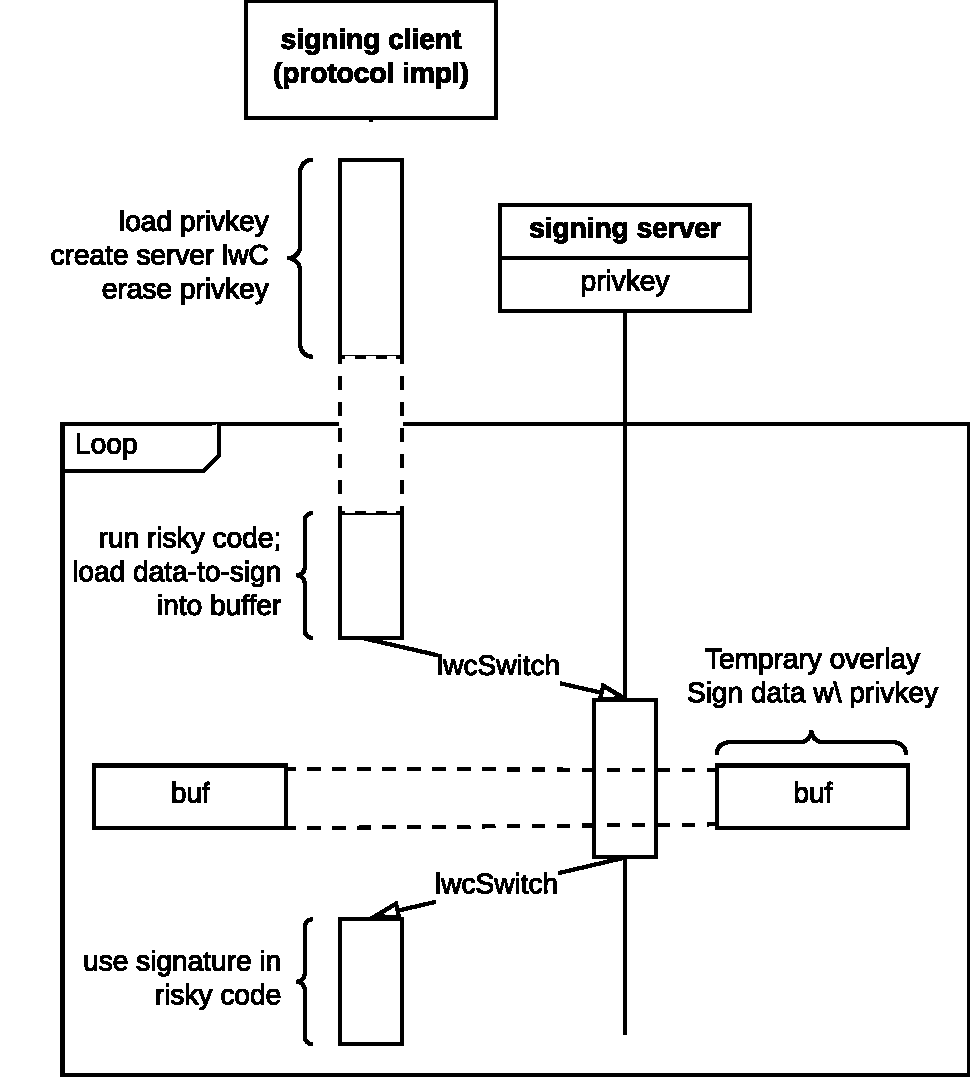
\includegraphics[height=4cm]{fig/encryption-compartment}
  \caption{
    TODO FULL WIDTH a)  b) comparison as described in Example Use Case section
  }
\end{figure}

Note that we have constructed a simplified example where requests can be handled in full isolation.
In practice, some sharing will be required, e.g., for global statistics, a database connection pool, logging services, etc.
In an lwC-compartmentalized design, these components would exectute in separate lwCs and be made accessible to the worker lwCs via shared memory, \lstinline{lwcSwitch}, \lstinline{lwcOverlay} or traditional IPC mechanisms.

Note further that we have not discussed the concurrency model of \appname: both threaded and event-driven models are possible, as will be shown in the evaluation (section~\ref{eval}).


\section{Implementation}\label{impl}

The authors implement light-weight contexts in the FreeBSD 11.0 operating system and make the source code publicly available.~\cite{lwckernelrepo,lwclibsrepo} % see literature.bib for git diff
The major changes to the kernel consist of:
\begin{itemize}
  \item An implementation of syscall handlers and resource specifier logic (+2388 lines in \texttt{sys/sys/kern\_snap.c}).
  \item Support for resource specifiers and overlays in
    file descriptor management (\lstinline{struct filedesc}, +251 lines in \texttt{sys/kern/kern\_descrip.c})
    and memory management subsystem  (+693 lines in \texttt{sys/vm/vm\_map.c}, +178 lines in \texttt{sys/amd64/amd64/pmap.c}).
  \item Platform-dependent code for \lstinline{lwcSwitch} (+250 lines in \texttt{sys/amd64/amd64/cpu\_switch.S}, +171 lines in \texttt{sys/amd64/amd64/vm\_machdep.c}).
\end{itemize}

User-space support for lwCs is provided through a C~library containing syscall wrappers and a synchronized hash-table that enables key-value sharing across lwCs.
The authors also provide a PHP extension that makes the lwC API accessible from scripts, which is requried for the evaluation.~\cite{lwclibsrepo}

\section{Evaluation}\label{eval}
The authors evaluate their implementation using micro-benchmarks to determine the primitive operations' latency
and integrate light-weight contexts into production applications, demonstrating its applicability and real-world performance impact.

\subsection{Micro-Benchmarks}
The micro-benchmarks first measure \lstinline{lwcSwitch} latency with regular context switching latency as the baseline, demonstrating a 2x speedup with negligible standard deviation.
While not explicitly stated, we assume that the measured \lstinline{lwcSwitch} is between lwCs with different address spaces.
The regular context switch is induced through a semaphore.

The overhead of creating and destroying lwCs is only given cummutatively: creating and immediately destroying a single lwC takes $87.7\mu s \approx 233282$ cycles on the evaluation machine. %(87.7*10^-6) * 2.66*10^9 = 233282
The authors do not provide a meaningful baseline, e.g., the latency of a forking and immediately exiting in the child.
An extended version of this micro-benchmark is also used to confirm that the run-time overhead within an lwC is limited to CoW faults, whose cost grow linearly with the amount of memory \lstinline{COPY}d on \lstinline{lwcCreate}.

The syscall interposition feature is evaluated by example:
the authors implement a reference monitor that intercepts the \lstinline{open}, \lstinline{read} and \lstinline{write} system calls, execute a dummy application that performs a fixed number of those system calls, and measure total execution time.
For comparison, they also measure a variant with inlined policy checks, as well as a variant that uses FreeBSD's Capsicum and multiple processes.
Thus, the result is the \textit{total execution time} per variant and system call, which is only useful to compare throughput, not latency.
Expectably, inlined policy checks exhibit the lowest overhead in all cases.
The context switching required for Capsicum and syscall interposition penalizes those variants on short syscalls (\lstinline{open}, small \lstinline{read} and \lstinline{write}).
For longer syscalls (large \lstinline{read}, \lstinline{write}), syscall interposition benefits from the \lstinline{mask} argument because copying the buffer to the reference monitor is not necessary.
\todo{figure helpful?}

\subsection{Application I: FastCGI Acceleration in PHP-FPM}
The authors integrate light-weight contexts into the PHP-FPM FastCGI server and adapt a Zend Hello-World application to use an lwC-enabled technique called \textit{snapshot-and-rollback}:
on first startup, before handling any request-specific data, the PHP script creates a snapshot of its initialized state using \lstinline{lwcCreate}.
This snapshot is then used as the basis for handling subsequent requests in a separate isolated lwCs which start execution at the pre-initialized state of the original snapshot.
Pseudocode for this operation is provided in figure~\ref{eval:phpfpm:pseudocode}.

\begin{lstlisting}[label=eval:phpfpm:pseudocode]
  SNAPSHOT-and-reload source code here
\end{lstlisting}

The authors compare the throughput of their snapshot-and-reload variant against upstream PHP-FPM, both with and without PHP opcode cache:
snapshot-and-reload achieves \textbf{2.7x throughput} if the opcode cache is disabled and \textbf{1.3x throughput} with enabled opcode cache.\todo{need to explain more verbosely why performance gain?}
Notably, this performance gain also comes with the security benefit of handling each request in a separate address space.

\subsection{Application II: Apache \& nginx with Session Isolation}
The authors also integrate light-weight contexts into the popular Apache and nginx web servers to protect TLS private keys and per-session data from attackers.
The Apache variant extends the Apache pre-fork concurrency mode, which uses dedicated threads per active client connection:
before a thread starts handling a new connection, it creates an lwC with private address space and file descriptor table and switches into it, thereby isolating potential attackers to a single thread in a dedicated lwC.
nginx implements an event-loop using non-blocking I/O with a single worker thread per core:
as with Apache, an lwC is created per connection but its descriptor is tracked in a hash map index by the socket file descriptor number.
When the kernel notifies the worker thread about pending I/O on a socket, the worker looks up the corresponding lwC and switches to it before resuming regular nginx request handling.
When socket I/O is reported to block, the worker switches back to the main event loop to handle other pending I/O.\todo{pending I/O comprehensible?}
Pseudocode for both Apache and nginx modifications is provided in figure~\ref{eval:web:pseudocode}.

\begin{lstlisting}
  Apache pseudocode

  Nginx pseudocode
\end{lstlisting}

The first set of benchmarks measures throughput of GET requests for a single 45 byte document at a constant number of concurrent clients.
The authors perform the experiment for different \textit{session lenghts}, i.e., the number of requests sent over a single connection using HTTP keep-alive.
For Apache, the lwC modifications exhibit significantly worse throughput for short sessions than stock pre-fork mode ($\ge80\%$ lower throughput).
16-request sessions, which we consider generous for highly interactive web applications, still exhibit $\approx 16\%$ lower throughput.
For nginx, performance implications are much less severe, with at most 22\% lower throughput for four-request sessions and at $\approx6\%$ lower throughput at 16-request sessions.
Our interpretation of the throughput improvements for Apache with growing session length is that the one-time additional latency for lwC creation and destruction is amortized for longer sessions.
However, this does not explain why nginx throughput is less-affected by lwCs, because nginx also creates an lwC per connection.

The authors also conduct a scalability experiment for nginx:
at a fixed session length of 256 requests, for 45 byte and 900 byte documents, the total throughput (GET/second) is measured for different numbers \todo{counts?} of concurrent clients.
For up to 6500 concurrent clients, there is no significant difference bewteen upstream nginx and lwC nginx.
For the 45 byte experiment, higher concurrency correlates with higher standard deviation and 19\% lower mean througput.
900 byte requests degrade more gracefully, with up to 10\% lower mean throughput at \~19500 concurrent clients.
The authors explain the sudden drop in performance at 6500 clients with CPU-bound behavior of an interrupt handler thread, which obviously affects both stock and modified nginx.




\subsection{Critique}\label{eval:crit}

% nice that is in fact applicable
% but:
% - PCID exhaustion not addressed in design & evaluation
% - benchmark scenario: single 44B file => nginx likely performs only 2 context switches

\section{Related Work}\label{rel}

\begin{itemize}
  \item Application Compartmentalization
  \begin{itemize}
    \item Principle of least Privilege
    
    \item Language-Technology-Based
    \begin{itemize}
      \item NaCL \& WASM
      \item BPF \& eBPF
      \item Software Fault Isolation
      \item Memory-safe Runtime (Java, CLR?) %working title, need proper PL word for it
    \end{itemize}
    
    \item OS-Based
      \begin{itemize}
        \item Capability Systems
        \begin{itemize}
          \item Fiasco-OC / seL4
          \item FreeBSD Capsicum
        \end{itemize}
        \item Process-Based Privsep
        \begin{itemize}
          \item Provos, OpenSSH
        \end{itemize}
        \item Hybrids (isolation at some level)
        \begin{itemize}
          \item wedge
          \item shreds (uses ARM memory domains)
          \item \textbf{light weight contexts}
        \end{itemize}
      \end{itemize}

    \item Hardware-Based
    \begin{itemize}
      \item CHERI
    \end{itemize}
  \end{itemize}
  
  \item Process Snapshotting \& Rollback
  \item Session Isolation in CGI applications?
\end{itemize}

\section{Conclusion}\label{conclusion}

% Cite all the literature, not just the one we referenced in the text.
\nocite{*}
\clearpage
\printbibliography

\end{document}
